\capitulo{3}{Conceptos teóricos}

En la presente sección se describen los principales conceptos teóricos con los que se ha trabajado a lo largo del proyecto. Estos fundamentos teóricos permitirán una mejor comprensión del producto final.

\section{Generación procedimental}
La generación procedimental, es la generación algorítmica de contenido de forma automática. Se podría decir en otras palabras que se refiere a un software que puede crear contenido de forma independiente sin necesidad de una persona que lo diseñe~\cite{proceduralgenbooknoor}.

Este concepto, si lo aplicamos a un videojuego, implica generar contenido de forma ilimitada, sin necesidad de un diseñador. El contenido que se puede generar abarca desde texturas, mapas, niveles, historias, música, armas, personajes, etc. Surgió para reducir costes y tiempo de desarrollo y para proporcionar una experiencia de juego única.

\subsection{Origen y ejemplos}
Los primeras aplicaciones de la generación procedimental en videojuegos se remonta a las primeras décadas del desarrollo de software de entretenimiento; había falta de recursos de almacenamiento y se necesitaban métodos eficientes para poder crear grandes volúmenes de contenido. Uno de los primeros juegos en usar generación procedimental es \textbf{<<Rogue>>}(1980). En este juego se usaba la generación procedimental para generar niveles de mazmorra de forma aleatoria en cada partida, así se podía obtener una experiencia completamente distinta en cada sesión, como se muestra en la figura \ref{fig:CaputraRogue}~\cite{proceduralgenbooknoor}.
\begin{figure}[h!]  
    \centering  
    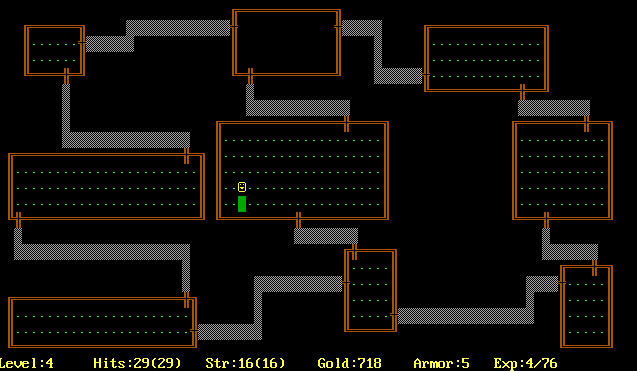
\includegraphics[width=\textwidth]{img/Rogue_Captura.PNG}  
    \caption{Captura del juego <<Rogue>>. Extraída de \url{https://es.wikipedia.org/wiki/Rogue.}}  
    \label{fig:CaputraRogue}
\end{figure}

\textbf{<<Minecraft>>} es otro ejemplo de juego que utiliza generación procedimental para los mapas. En el caso de este juego los mundos se generan de forma procedimental usando la función matemática \textbf{<<Ruido Perlin>>}\footnote{El <<Ruido Perlin>> hace uso de una interpolación entre un gran número de gradientes precalculados, construyen de esta forma un valor que varía, similar al ruido blanco y se utiliza para generar imágenes.\cite{wikipediaPerlin}} modificado, de esta forma crea terrenos, biomas y cuevas únicas cada vez que se inicia el juego. Esto permite crear un mundo muy extenso y variado sin la necesidad de diseñarlos manualmente~\cite{proceduralgenbooknoor}.

Pero el mejor ejemplo de juego procedimental es \textbf{<<No Man's Sky>>}. Este juego consigue crear mundos y universos de forma procedimental. A través de multitud de algoritmos complejos consigue crear planetas enteros, incluyendo la flora, fauna y paisajes, como se muestra en la figura \ref{fig:CaputraNoMansSky}. Este juego proporciona una experiencia de exploración infinita, esta capacidad de generación procedimental ha permitido a este juego crear un entorno expansivo que no se podría crear manualmente~\cite{proceduralgenbooknoor}.
\begin{figure}[h!]  
    \centering  
    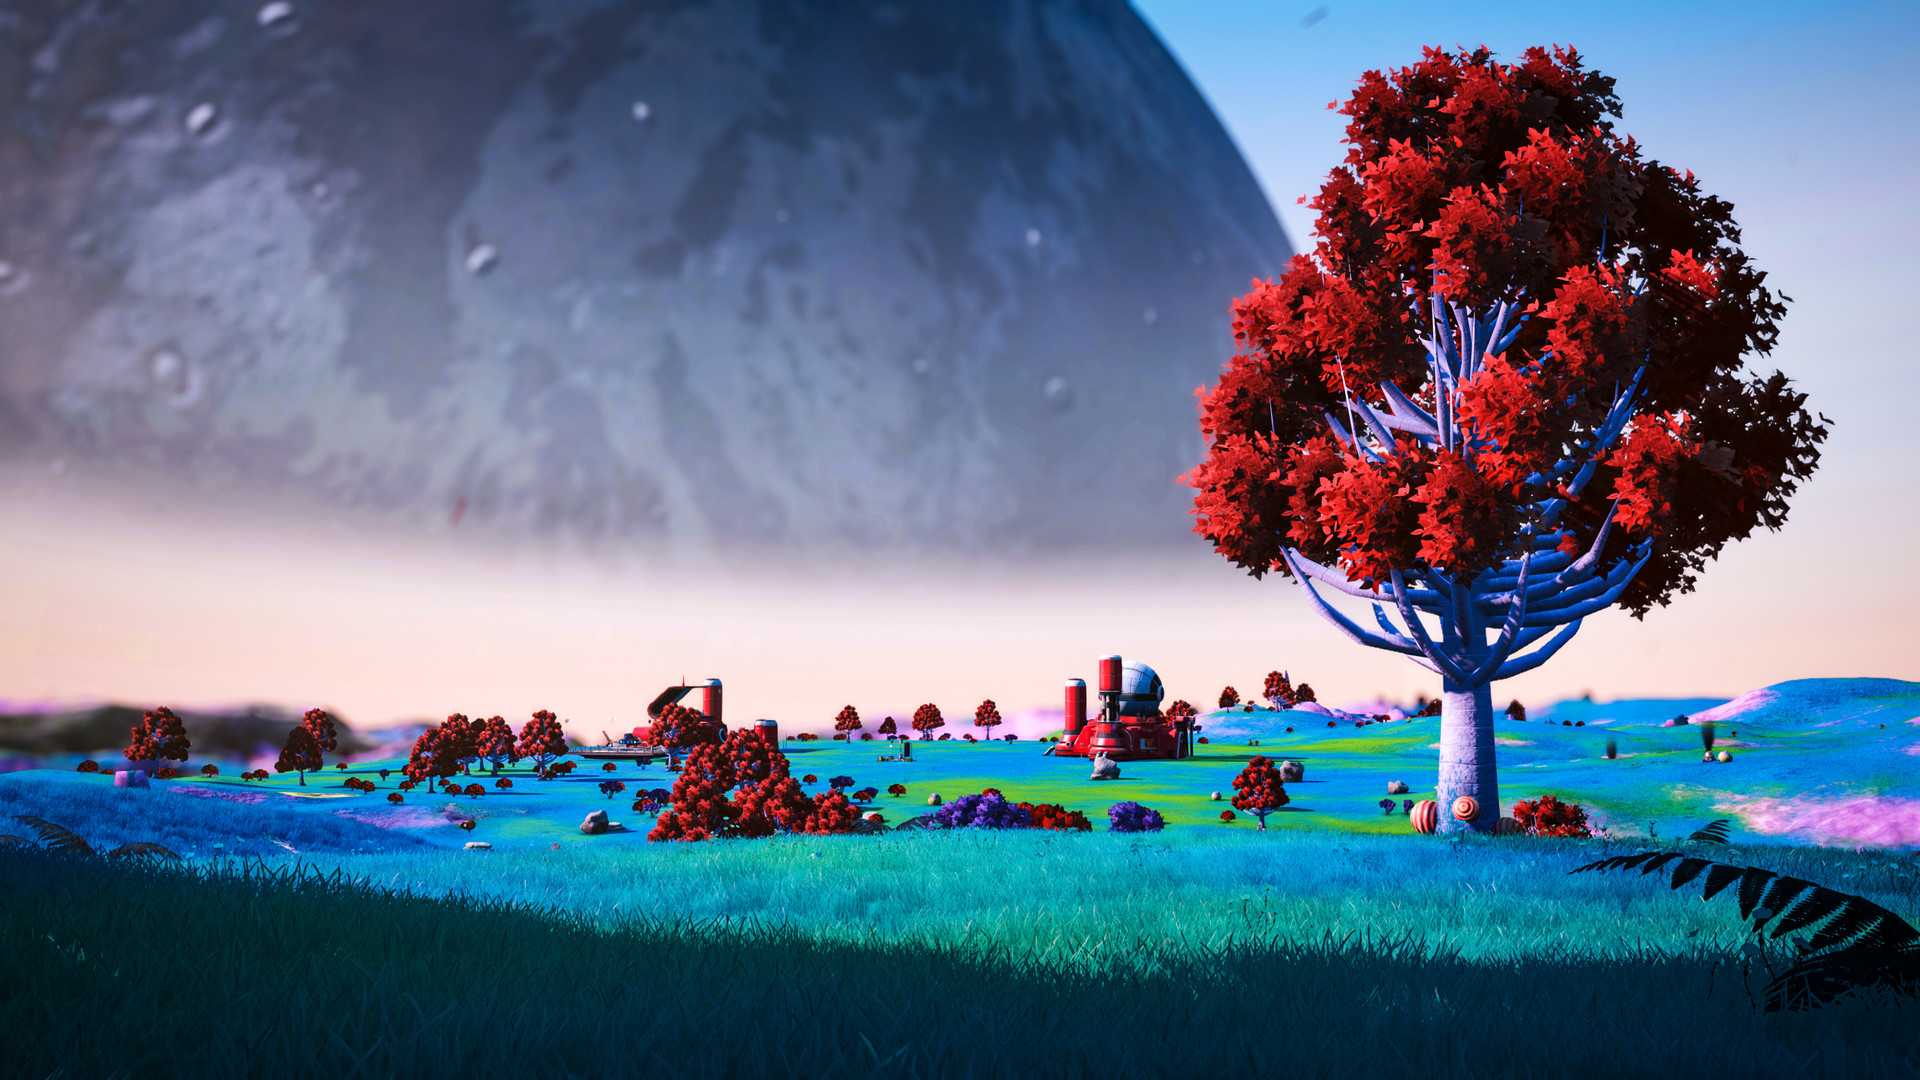
\includegraphics[width=\textwidth]{img/NoMansSkyScreenShot.jpg}  
    \caption{Captura del juego <<No Man's Sky>>. Extraída de \url{https://www.artstation.com/artwork/gEZ9P?album_id=660885}}  
    \label{fig:CaputraNoMansSky}
\end{figure}

\section{Algoritmos}
\subsection{Algoritmo de Prim}
El algoritmo de Prim, se ha usado tradicionalmente para encontrar el árbol de expansión mínima en un grafo, esto se puede adaptar para generar laberintos. Para adaptarlo, se seleccionan caminos aleatoriamente desde una celda inicial, y se va a expandir de forma que se mantenga la conectividad del laberinto sin crear ciclos, creando un camino único entre cualquier par de celdas~\cite{MazeGenAnalysis}.

Para poder generar el laberinto, en este caso el algoritmo se ha adaptado usando un enfoque que expande caminos desde una celda inicial y agrega aleatoriamente celdas vecinas a la estructura del laberinto. Así se puede asegurar de que se mantienen caminos únicos entre celdas, no se crean ciclos innecesarios y se genera un laberinto completamente conectado sin caminos redundantes. Funciona de una forma similar a cómo tradicionalmente se selecciona el arista más barato para expandir el árbol en un grafo.


\begin{algorithm}
\caption{Algoritmo DungeonPrim}
\begin{algorithmic}[1]
\Require Ancho $w$, alto $h$, semilla $s$ (opcional)
\Ensure Generar un laberinto usando el algoritmo de Prim

\State Inicializar la cuadrícula de mazmorra con tamaño $w \times h$
\If{$s \neq \text{None}$}
    \State Establecer semilla aleatoria $s$
\EndIf

\State Elegir una celda inicial $start$ aleatoria
\State Cambiar estado de $start$ a \texttt{PATH}
\State Agregar posición de $start$ a $steps$
\State $frontier\_set \gets$ vecinos de $start$ a distancia 2

\While{$frontier\_set$ no esté vacío}
    \State Elegir una celda $frontier\_cell$ aleatoria de $frontier\_set$
    \State Eliminar $frontier\_cell$ de $frontier\_set$

    \State \small{$frontier\_neighs \gets$ vecinos de $frontier\_cell$ a distancia 2 que sean \texttt{PATH}}
    \State Elegir una celda $connect\_cell$ aleatoria de $frontier\_neighs$

    \State Cambiar estado de $frontier\_cell$ a \texttt{PATH}
    \State Agregar posición de $frontier\_cell$ a $steps$

    \State Cambiar estado de la celda entre $frontier\_cell$ y $connect\_cell$ a \texttt{PATH}

    \State $new\_neighbors \gets$ vecinos de $frontier\_cell$ a distancia 2 que sean \texttt{WALL}
    \State Agregar $new\_neighbors$ a $frontier\_set$
\EndWhile

\State Definir $exit$ como la última celda conectada

\end{algorithmic}
\end{algorithm}


\subsection{Depth First Search-DFS}
El algoritmo de búsqueda de profundidad (DFS) es un algoritmo que se utiliza en la teoría de grafos y en árboles, para buscar caminos y soluciones en profundidad antes de retroceder. Este algoritmo se puede adaptar para crear laberintos con múltiples caminos y conexiones, asegurando que va a haber una solución de navegación sin realizar ciclos innecesarios~\cite{MazeGenAnalysis}.

En este caso, desde la celda inicial, el algoritmo explora en profundidad antes de retroceder y probar otro camino, y se crea un camino marcando las celdas como parte del laberinto mientras elimina los muros entre celdas adyacentes.
Los vecinos se barajan aleatoriamente para asegurar que el laberinto generado tenga una estructura impredecible y no se vean patrones evidentes.

\begin{algorithm}
\caption{Algoritmo DungeonDFS}
\begin{algorithmic}[1]
\Require Ancho $w$, alto $h$, semilla $s$ (opcional)
\Ensure Generar laberintos usando búsqueda en profundidad (DFS)

\State Inicializar la cuadrícula de mazmorra con tamaño $w \times h$
\If{$s \neq \text{None}$}
    \State Establecer semilla aleatoria $s$
\EndIf

\State Elegir una celda inicial $start$ aleatoria
\State Llamar a \texttt{hacer\_caminos($start$)}

\Procedure{hacer\_caminos}{cell, from\_cell}
    \State Cambiar estado de $cell$ a \texttt{PATH}
    \If{from\_cell $\neq$ None}
        \State Cambiar estado de la celda entre $cell$ y $from\_cell$ a \texttt{PATH}
        \State Agregar posición de la celda intermedia a $steps$
    \EndIf

    \State Obtener vecinos $random\_neighs$ de $cell$ a distancia 2
    \State Mezclar aleatoriamente $random\_neighs$

    \For{neigh en $random\_neighs$}
        \State Definir $exit$ como $neigh$
        \If{$neigh.state = \text{PATH}$}
            \State \textbf{continuar}
        \EndIf
        \State Llamar a \texttt{hacer\_caminos($neigh$, $cell$)}
    \EndFor
\EndProcedure

\Function{obtener\_celda\_entre}{origin, target}
    \State $(row\_origin, col\_origin) \gets origin.\text{get\_position}()$
    \State $(row\_target, col\_target) \gets target.\text{get\_position}()$

    \If{$row\_origin = row\_target$}
        \State \Return grid[$row\_origin$][max($col\_origin$, $col\_target$) - 1]
    \Else
        \State \Return grid[max($row\_origin$, $row\_target$) - 1][$col\_origin$]
    \EndIf
\EndFunction

\end{algorithmic}
\end{algorithm}



\subsection{Autómata celular}
Un autómata celular es un modelo matemático que se compone por una cuadrícula de celdas, cada una de las celdas puede estar en un estado finito, uno o cero. Esta cuadrícula va a evolucionar a lo largo de una serie de iteraciones, en el que el estado de cada celda en la siguiente iteración se determina en función de su estado actual y las celdas vecinas según unas reglas locales y uniformes. Para que pueda comenzar, se necesita proveer un estado inicial al algoritmo~\cite{cellularAutomata}.

Es similar a <<El juego de la vida>> de Conway, en el que las celdas van evolucionando a lo largo del tiempo en función de una serie de reglas y se va cambiando su estado de viva a muerta~\cite{wikipediaMazeGeneration}.


En este caso se ha adaptado de forma que en cada iteración se crea una nueva cuadrícula basada en la cuadrícula actual. Para comenzar, se le provee de unas celdas en estado de camino al algoritmo. Tras ese crea una copia de la cuadrícula actual para no modificar la cuadrícula original durante la iteración. Después para cada celda se contabilizan los vecinos que son muros y si la celda tiene más de 4 o menos de 1 vecino que es muro, se convierte en un camino, si la celda tiene 3 vecinos que son muros, se convierte en muro.


\begin{algorithm}
\caption{Algoritmo DungeonCellular}
\begin{algorithmic}[1]
\Require Ancho $w$, alto $h$, semilla $s$ (opcional), iteraciones máximas $max\_iterations$ (opcional), puntos de inicio $starting\_points$ (opcional)
\Ensure Generar laberintos usando un autómata celular

\State Inicializar la cuadrícula de mazmorra con tamaño $w \times h$ y todas las celdas como \texttt{PATH}
\If{$s \neq \text{None}$}
    \State Establecer semilla aleatoria $s$
\Else
    \State Establecer una semilla aleatoria
\EndIf

\State $iters \gets max\_iterations$ o $(w \times h) / 2$
\If{$starting\_points$ está vacío}
    \State Generar puntos de inicio aleatorios y establecer como \texttt{WALL}
\Else
    \For{cada punto en $starting\_points$}
        \State Establecer punto como \texttt{WALL}
    \EndFor
\EndIf

\For{$i \gets 1$ hasta $iters$}
    \State Crear una nueva cuadrícula basada en las reglas de vecindad:
    \For{cada celda en la cuadrícula}
        \State Calcular el número de vecinos \texttt{WALL}
        \If{$num\_neigh > 4$ o $num\_neigh < 1$}
            \State Cambiar estado de la celda a \texttt{PATH}
        \ElsIf{$num\_neigh = 3$}
            \State Cambiar estado de la celda a \texttt{WALL}
        \EndIf
    \EndFor
\EndFor

\end{algorithmic}
\end{algorithm}



\subsection{Algoritmo de Eller}
El algoritmo de Eller es un método de generación de laberintos basado en la creación de conjuntos de celdas. Se procesa una fila cada vez, haciendo que todas las celdas estén conectadas de alguna manera. Se utiliza para generar laberintos en tiempo real o de manera infinita horizontalmente~\cite{MazeGenAnalysis}.

En este algoritmo se necesita hacer uso de la estructura de datos \textbf{Union-Find} o estructura de conjuntos disjuntos, se utiliza para gestionar y unir subconjuntos de elemento y para ver si dos elementos forman parte del mismo conjunto.

Para este caso se ha adaptado, de forma que cada celda comienza en un conjunto separado. Según se van procesando las filas, las celdas se agrupan en conjuntos que se unen de forma horizontal y vertical, asegurando así que todas las celdas estén conectadas al final. 
En cada fila, las celdas adyacentes se agrupan aleatoriamente si pertenecen a conjuntos distintos, creando así pasajes horizontales. Para crear conexiones verticales aleatorias, se hacen de forma aleatoria entre filas, asegurando que los conjuntos se conectan a la siguiente fila, así el laberinto va a tener caminos continuos de una fila a la siguiente.

\begin{algorithm}
\caption{Algoritmo DungeonEller}
\begin{algorithmic}[1]
\Require Ancho $w$, alto $h$, semilla $s$ (opcional)
\Ensure Generar laberintos usando el algoritmo de Eller

\State Inicializar la cuadrícula de mazmorra con tamaño $w \times h$
\If{$s \neq \text{None}$}
    \State Establecer semilla aleatoria $s$
\EndIf

\For{cada fila impar $row\_index$ desde 1 hasta $h-2$}
    \State Obtener fila $row$
    \State Crear conjuntos para las celdas en $row$
    \State Agrupar celdas adyacentes en $row$
    \State Obtener la siguiente fila $next\_row$
    \State Crear conexiones verticales aleatorias entre $row$ y $next\_row$
\EndFor

\State Obtener la última fila $last\_row$
\State Crear conjuntos para las celdas en $last\_row$
\State Agrupar celdas adyacentes en $last\_row$

\Procedure{crear\_conjuntos}{row}
    \For{cada celda en $row$}
        \If{celda no tiene conjunto}
            \State Crear nuevo conjunto para la celda
        \EndIf
    \EndFor
\EndProcedure

\Procedure{crear\_conexiones\_verticales}{row, next\_row}
    \State Obtener posibles conexiones verticales
    \State Mezclar aleatoriamente las conexiones
    \For{cada conexión seleccionada}
        \State Unir conjuntos de las celdas conectadas
        \State Conectar las celdas
    \EndFor
\EndProcedure

\Procedure{agrupar\_adyacentes}{row}
    \For{cada par de celdas adyacentes en $row$}
        \If{celdas no están en el mismo conjunto}
            \State Unir conjuntos y conectar celdas
        \EndIf
    \EndFor
\EndProcedure

\end{algorithmic}
\end{algorithm}




\subsection{Algoritmo de Kruskal}
El algoritmo de Kruskal es un algoritmo de grafos que se utiliza para encontrar el árbol de expansión mínima en un grafo no dirigido. El objetivo es encontrar un subconjunto de aristas del grafo que conectan todos los vértices sin ciclos y con el menor peso total posible~\cite{MazeGenAnalysis}.

Para generar laberintos, este algoritmo se adapta para conectar todas las celdas sin crear ciclos, garantizando un camino único entre cualquier par de celdas.
Cada celda empieza en un conjunto independiente. Según se procesan las aristas, las celdas se unen entre sí únicamente si no pertenecen al mismo conjunto, fusionando ambos conjuntos. De esta forma, sólo hay un camino sin ciclos. Las aristas se seleccionan de forma aleatoria, así se pueden evitar patrones previsibles y que el resultado sea impredecible, haciendo que en este sentido sea similar a DFS. 

Para poder trabajar con los conjuntos, al igual que con Eller, se hace uso de la estructura de datos Union-Find, mencionada en el anterior apartado.  

\begin{algorithm}
\caption{Algoritmo DungeonKruskal}
\begin{algorithmic}[1]
\Require Ancho $w$, alto $h$, semilla $s$ (opcional)
\Ensure Generar laberintos usando el algoritmo de Kruskal

\State Inicializar la cuadrícula de mazmorra con tamaño $w \times h$
\If{$s \neq \text{None}$}
    \State Establecer semilla aleatoria $s$
\EndIf

\State Inicializar lista de celdas $flattened\_maze$
\State Inicializar lista de aristas $edges$

\For{cada celda en posiciones impares de la cuadrícula}
    \State Agregar celda a $flattened\_maze$
\EndFor
\For{cada fila impar excepto la última}
    \For{cada columna impar excepto la última}
        \State Agregar arista vertical y horizontal a $edges$
    \EndFor
\EndFor
\For{cada columna impar de la última fila}
    \State Agregar arista horizontal a $edges$
\EndFor
\State Inicializar estructura Union-Find con $flattened\_maze$
\State Mezclar aleatoriamente las aristas en $edges$

\While{$edges$ no esté vacío}
    \State Obtener y remover una arista $(A, B)$ de $edges$
    \If{A y B no están en el mismo conjunto}
        \State Conectar celdas $A$ y $B$ en la cuadrícula
        \State Unir conjuntos de $A$ y $B$ en Union-Find
    \EndIf
\EndWhile
\Procedure{conectar\_celdas}{A, B}
    \State Obtener celda entre $A$ y $B$
    \State Cambiar estado de la celda intermedia a \texttt{PATH}
    \State Cambiar estado de $A$ y $B$ a \texttt{PATH}
\EndProcedure
\end{algorithmic}
\end{algorithm}




\subsection{Teselación}
La teselación, es el proceso de cubrir un plano con una o más formas geométricas, denominadas teselas. De esta forma se consigue que no queden espacios ni se superpongan. Para aplicarlo a la generación de laberintos, se utilizan patrones que se van a repetir y combinar para crear un laberinto continuo y complejo~\cite{wikipediaMazeGeneration}.

Se comienza con una pequeña sección de laberinto que incluye caminos, esta será la base de la iteración. En cada iteración, la cuadrícula se duplica tanto horizontal como verticalmente, haciendo una cuadrícula más grande que tiene varias copias de la original. Después se seleccionan aperturas al azar en los muros de la cuadrícula original para mantener la conectividad entre las secciones duplicadas, asegurándose de que ninguna sección esté aislada. 

Debido a la naturaleza de este algoritmo, no es posible personalizar las dimensiones del laberinto dados unos parámetros determinados.


\begin{algorithm}
\caption{Algoritmo DungeonTesselation}
\begin{algorithmic}[1]
\Require Iteraciones $iters$, semilla $s$ (opcional)
\Ensure Generar laberintos usando el algoritmo de teselación

\State Inicializar la cuadrícula con una estructura base de 3x3
\If{$s \neq \text{None}$}
    \State Establecer semilla aleatoria $s$
\EndIf

\For{cada iteración desde 1 hasta $iters$}
    \State Llamar a \texttt{teselación()}
\EndFor

\Procedure{teselación}{}
    \State Obtener tamaño anterior de la cuadrícula $pre\_size\_x$ y $pre\_size\_y$
    \State Duplicar filas y columnas de la cuadrícula

    \State Inicializar lista de aperturas $appertures$
    \State Agregar aperturas horizontales y verticales a $appertures$
    \State Mezclar aleatoriamente $appertures$
    \State Remover una apertura aleatoriamente

    \For{cada apertura en $appertures$}
        \State Cambiar estado de la celda a \texttt{PATH}
    \EndFor
\EndProcedure

\Function{verificar\_apertura\_vertical}{y, x}
    \If{fuera de límites verticales}
        \State \Return False
    \EndIf
    \State \Return ambas celdas adyacentes verticalmente son \texttt{PATH}
\EndFunction

\Function{verificar\_apertura\_horizontal}{y, x}
    \If{fuera de límites horizontales}
        \State \Return False
    \EndIf
    \State \Return ambas celdas adyacentes horizontalmente son \texttt{PATH}
\EndFunction

\end{algorithmic}
\end{algorithm}



\clearpage 

\subsection{Algoritmo de Aldous Broder}
El algoritmo de Aldous Broder es un algoritmo que se utiliza para generar laberintos, lo hace a través de un recorrido aleatorio para visitar todas las celdas del laberinto. Es de los algoritmos más sencillos de implementar, pero ineficientes, ya que visita la misma celda múltiples veces, hasta encontrar una celda que no ha sido visitada. Pero al ser aleatorio, es útil para crear laberintos que carezcan de patrones repetitivos~\cite{MazeGenAnalysis}.

Primero se elige una celda vecina de la casilla inicial de forma aleatoria, y se mueve a ella. La celda vecina si aún es un muro, se crea un pasaje entre ambas celdas quitando el muro y la celda vecina pasa a ser la celda a la que se va a apuntar. Sobre la celda que se apunta se vuelve a seleccionar un vecino aleatoriamente, y se comprueba si se ha visitado o no. En este caso se necesita adaptar la comprobación de vecinos a una distancia de dos celdas ya que los muros ocupan lo mismo que un camino. Este proceso se va repitiendo hasta completar el laberinto, por eso en laberintos de grandes dimensiones es muy ineficiente.



\begin{algorithm}
\caption{Algoritmo DungeonAldousBroder}
\begin{algorithmic}[1]
\Require Ancho $w$, alto $h$, semilla $s$ (opcional)
\Ensure Generar laberintos usando el algoritmo de Aldous Broder

\State Inicializar la cuadrícula de mazmorra con tamaño $w \times h$
\If{$s \neq \text{None}$}
    \State Establecer semilla aleatoria $s$
\EndIf

\State Inicializar lista de celdas no visitadas $unvisited\_cells$
\State Elegir una celda inicial aleatoria $current\_cell$ de $unvisited\_cells$
\State $remaining\_cells \gets$ número de celdas no visitadas

\While{$remaining\_cells > 0$}
    \If{$current\_cell$ es \texttt{WALL}}
        \State Cambiar estado de $current\_cell$ a \texttt{PATH}
        \State $remaining\_cells \gets remaining\_cells - 1$
    \EndIf
    \State Elegir una nueva celda aleatoria $new\_cell$ de los vecinos de $current\_cell$
    \If{$new\_cell$ es \texttt{WALL}}
        \State Conectar $current\_cell$ con $new\_cell$
    \EndIf
    \State $current\_cell \gets new\_cell$
\EndWhile

\Procedure{conectar\_celdas}{origin, target}
    \State Obtener posición de $origin$ y $target$
    \If{la distancia es vertical}
        \State Conectar celdas verticalmente
    \Else
        \State Conectar celdas horizontalmente
    \EndIf
    \State Cambiar estado de las celdas conectadas a \texttt{PATH}
\EndProcedure

\end{algorithmic}
\end{algorithm}




\subsection{Árbol Binario}
Un árbol binario es una estructura de datos.
El algoritmo para generar laberintos se adapta de forma que en una cuadrícula cada celda tenga como máximo dos conexiones. Esto da como resultado laberintos con un patrón donde hay muchos caminos que llevan a la celda de inicio, y no se crean ciclos en el laberinto generado~\cite{wikipediaMazeGeneration}.

Para adaptar este algoritmo, se va a recorrer la matriz de celdas en pasos de dos, creando un laberinto donde cada celda va a tener como máximo dos conexiones. Para cada celda, se conectan horizontal o verticalmente, haciendo que cada celda esté conectada a otra sin hacer ciclos, creando caminos únicos y continuos.




\begin{algorithm}
\caption{Algoritmo DungeonBinaryTree}
\begin{algorithmic}[1]
\Require Ancho $w$, alto $h$, semilla $s$ (opcional)
\Ensure Generar laberintos usando el Algoritmo de Árbol Binario

\State Inicializar la cuadrícula de mazmorra con tamaño $w \times h$
\If{$s \neq \text{None}$}
    \State Establecer semilla aleatoria $s$
\EndIf

\For{cada fila impar $row$ desde 1 hasta $h$}
    \For{cada columna impar $column$ desde 1 hasta $w$}
        \State Obtener celda actual $cell$
        \State Obtener celda superior $upper\_cell$
        \State Obtener celda derecha $right\_cell$
        
        \If{no hay celdas adyacentes}
            \State \textbf{continuar}
        \ElsIf{no hay celda superior}
            \State Conectar $cell$ con $right\_cell$
        \ElsIf{no hay celda derecha}
            \State Conectar $cell$ con $upper\_cell$
        \Else
            \State Conectar $cell$ con una celda aleatoria entre $upper\_cell$ y $right\_cell$
        \EndIf
    \EndFor
\EndFor

\Procedure{conectar\_celdas}{cell, target}
    \State Obtener posición de $cell$ y $target$
    \If{la distancia es vertical}
        \State Conectar celdas verticalmente
    \Else
        \State Conectar celdas horizontalmente
    \EndIf
    \State Cambiar estado de las celdas conectadas a \texttt{PATH}
\EndProcedure

\end{algorithmic}
\end{algorithm}



\section{Análisis de tiempos de ejecución}
Una forma de evaluar los algoritmos, es observar los tiempos de ejecución de cada uno de ellos. En este caso, se puede evaluar de todos excepto de los algoritmos de Teselación y Autómata Celular. 
En el caso del Autómata celular, se necesita un número de iteraciones por lo que no se puede medir la complejidad algorítmica, y en el caso de la Teselación, al no poder especificar unas dimensiones determinadas, no se puede realizar la comparación con el resto de algoritmos. Por ello se han hecho gráficas separadas para poder ver su evolución según los tiempos de ejecución, como se muestran en las figuras \ref{fig:TeselacionTiempos} y \ref{fig:CelularTiempos}.

En la figura \ref{fig:TeselacionTiempos}, que pertenece a la adaptación del algoritmo de Teselación, se puede observar que a partir de 9 iteraciones el tiempo de ejecución incrementa exponencialmente, por ello en la aplicación no se va a permitir generar laberintos a partir de 10 iteraciones, debido a que el tiempo que tardaría en generarlos sería excesivo.

La figura \ref{fig:CelularTiempos} refleja los tiempos de ejecución de la adaptación del algoritmo Autómata Celular. En esta gráfica se puede ver reflejado que a partir de las dimensiones 50x50 el tiempo de ejecución incrementa.

En la figura \ref{fig:TiemposAlgoritmos} se puede ver la cantidad de tiempo que tarda en generar laberintos de cierta dimensión. Resultados más detallados pueden verse en las tablas \ref{tab:resultados_detallados_parte1} y \ref{tab:resultados_detallados_parte2}.
Como se puede observar, el algoritmo más eficiente de todos es el árbol binario, teniendo la complejidad temporal más baja. El algoritmo más costo de todos es Eller, teniendo un resultado incrementalmente mayor respecto a los otros algoritmos al aumentar el tamaño de los laberintos, haciendo que sea el más complejo de todos~\cite{MazeGenAnalysis}.

\vspace{3cm}

\begin{figure}
    \centering  
    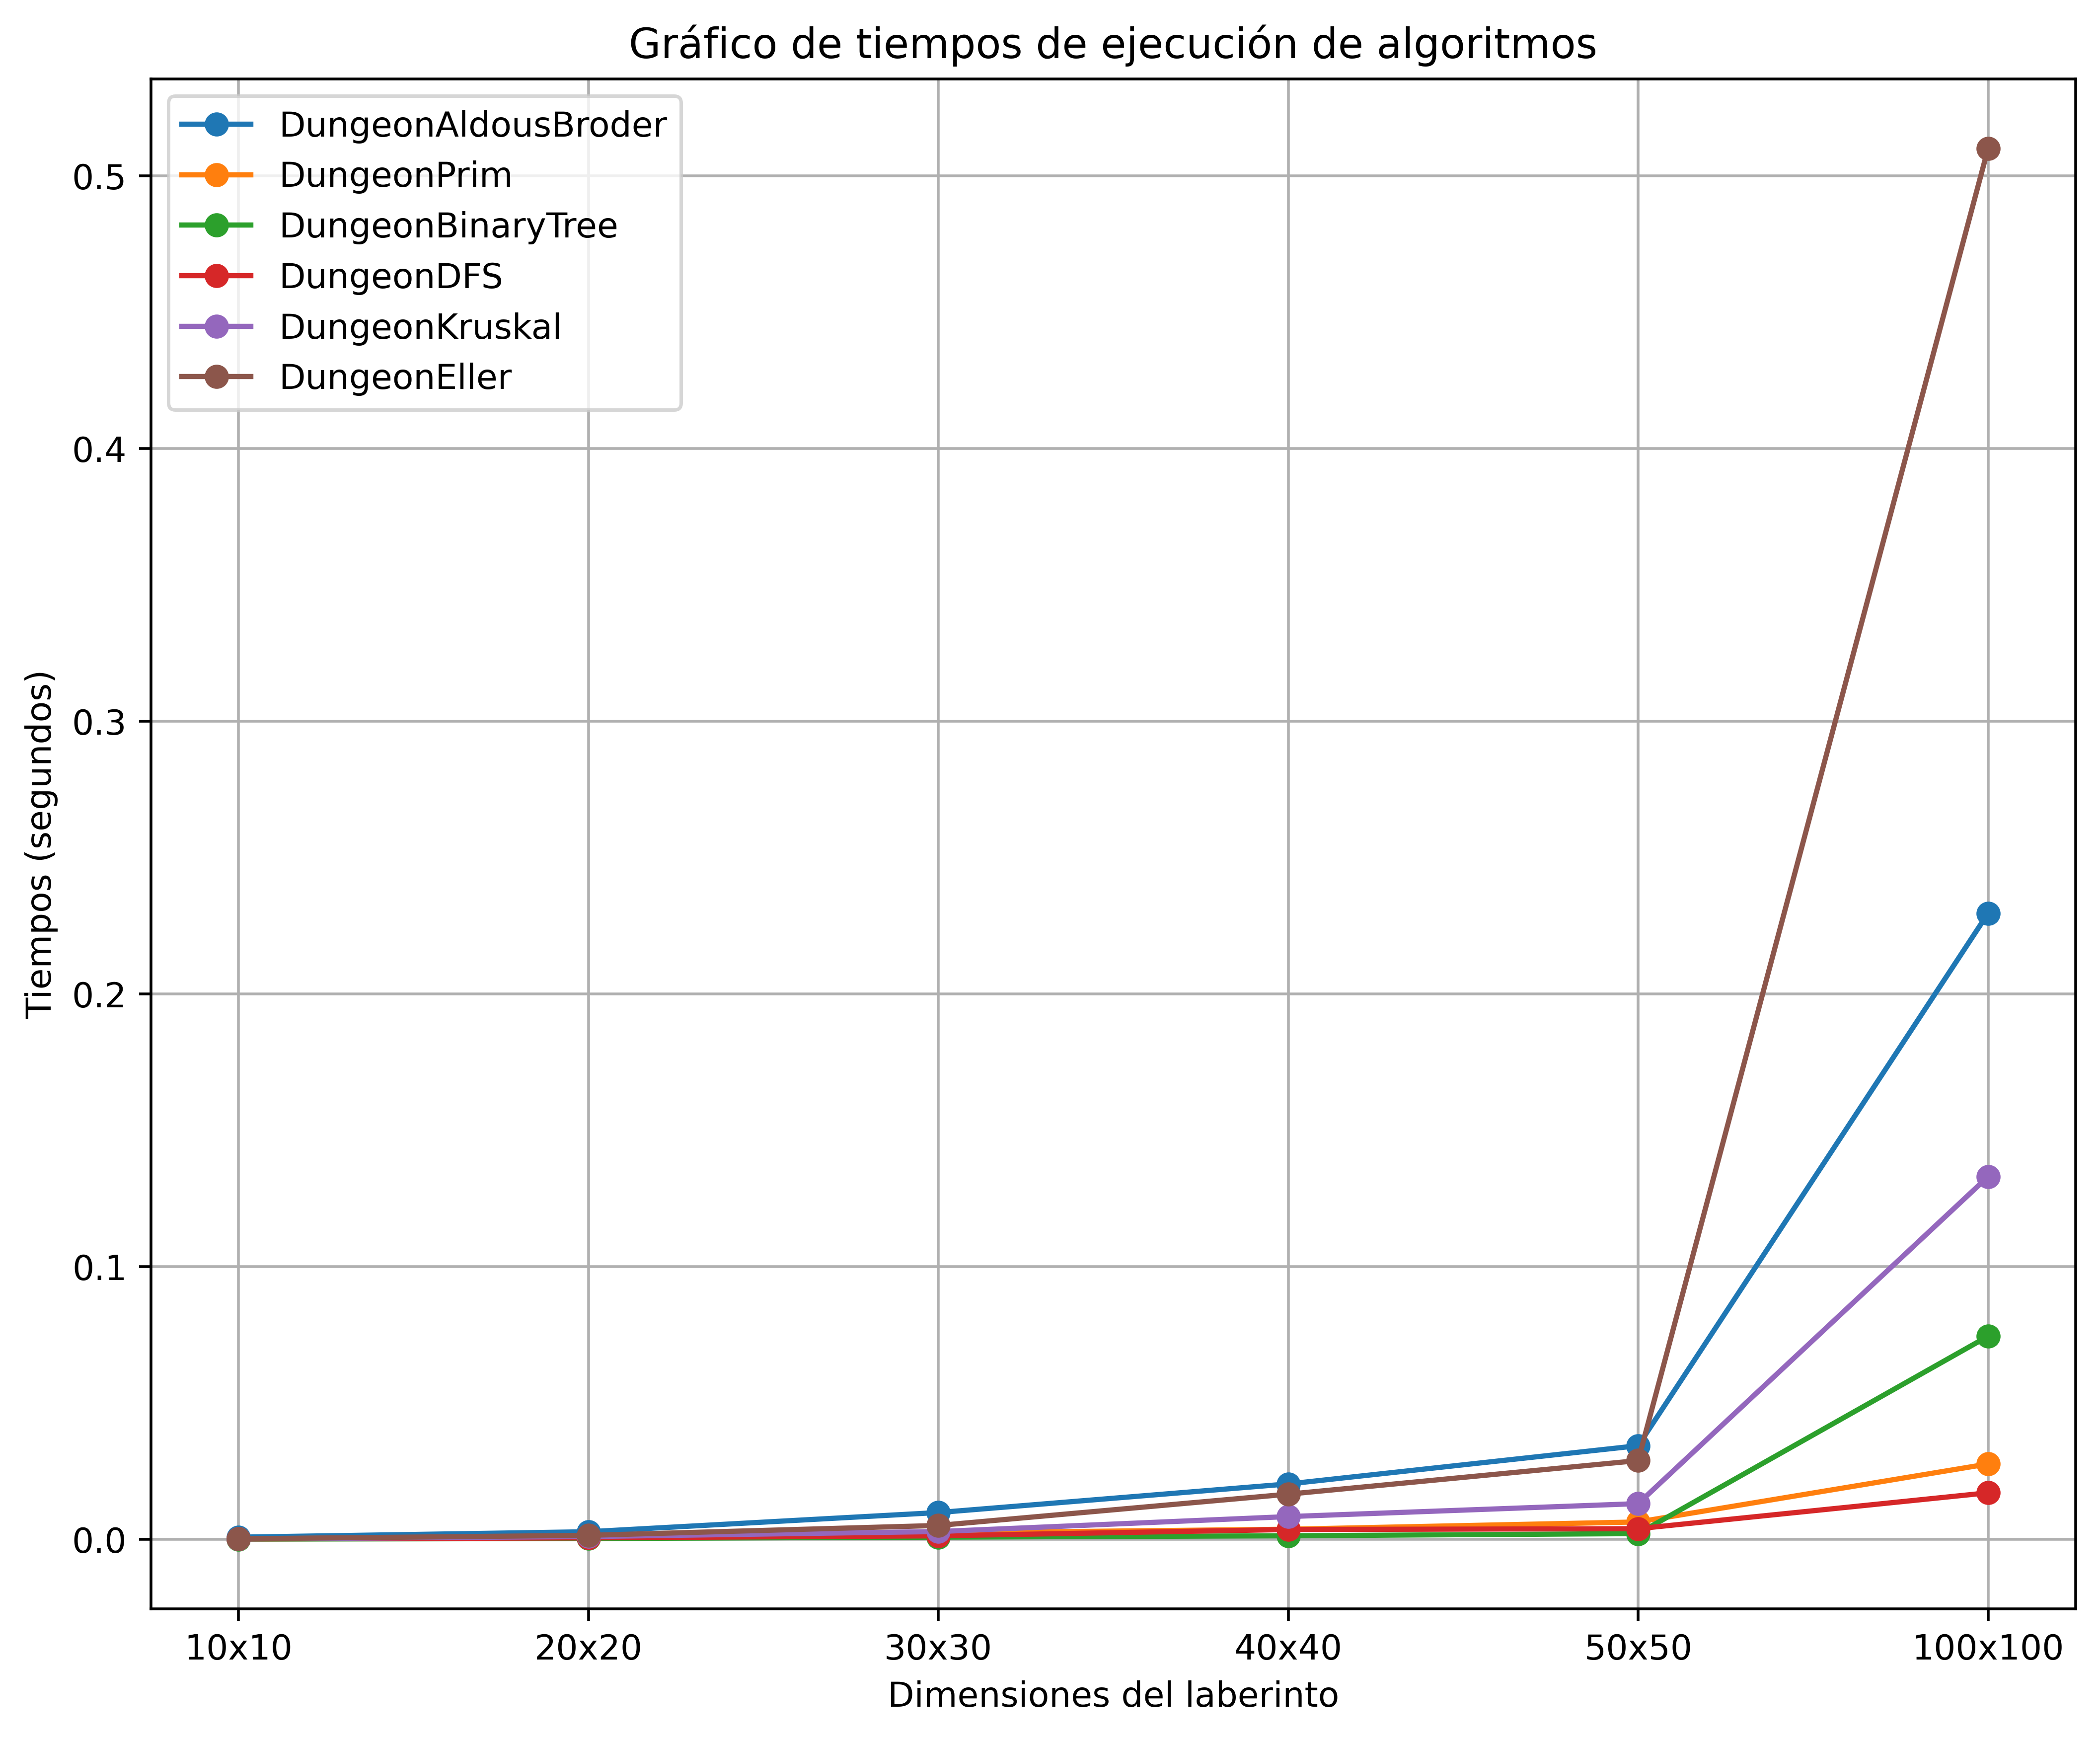
\includegraphics[width=\textwidth]{img/TimeGraph.png}  
    \caption{Gráfico de tiempos de ejecución de algoritmos}  
    \label{fig:TiemposAlgoritmos}
\end{figure}

\begin{figure}
    \centering  
    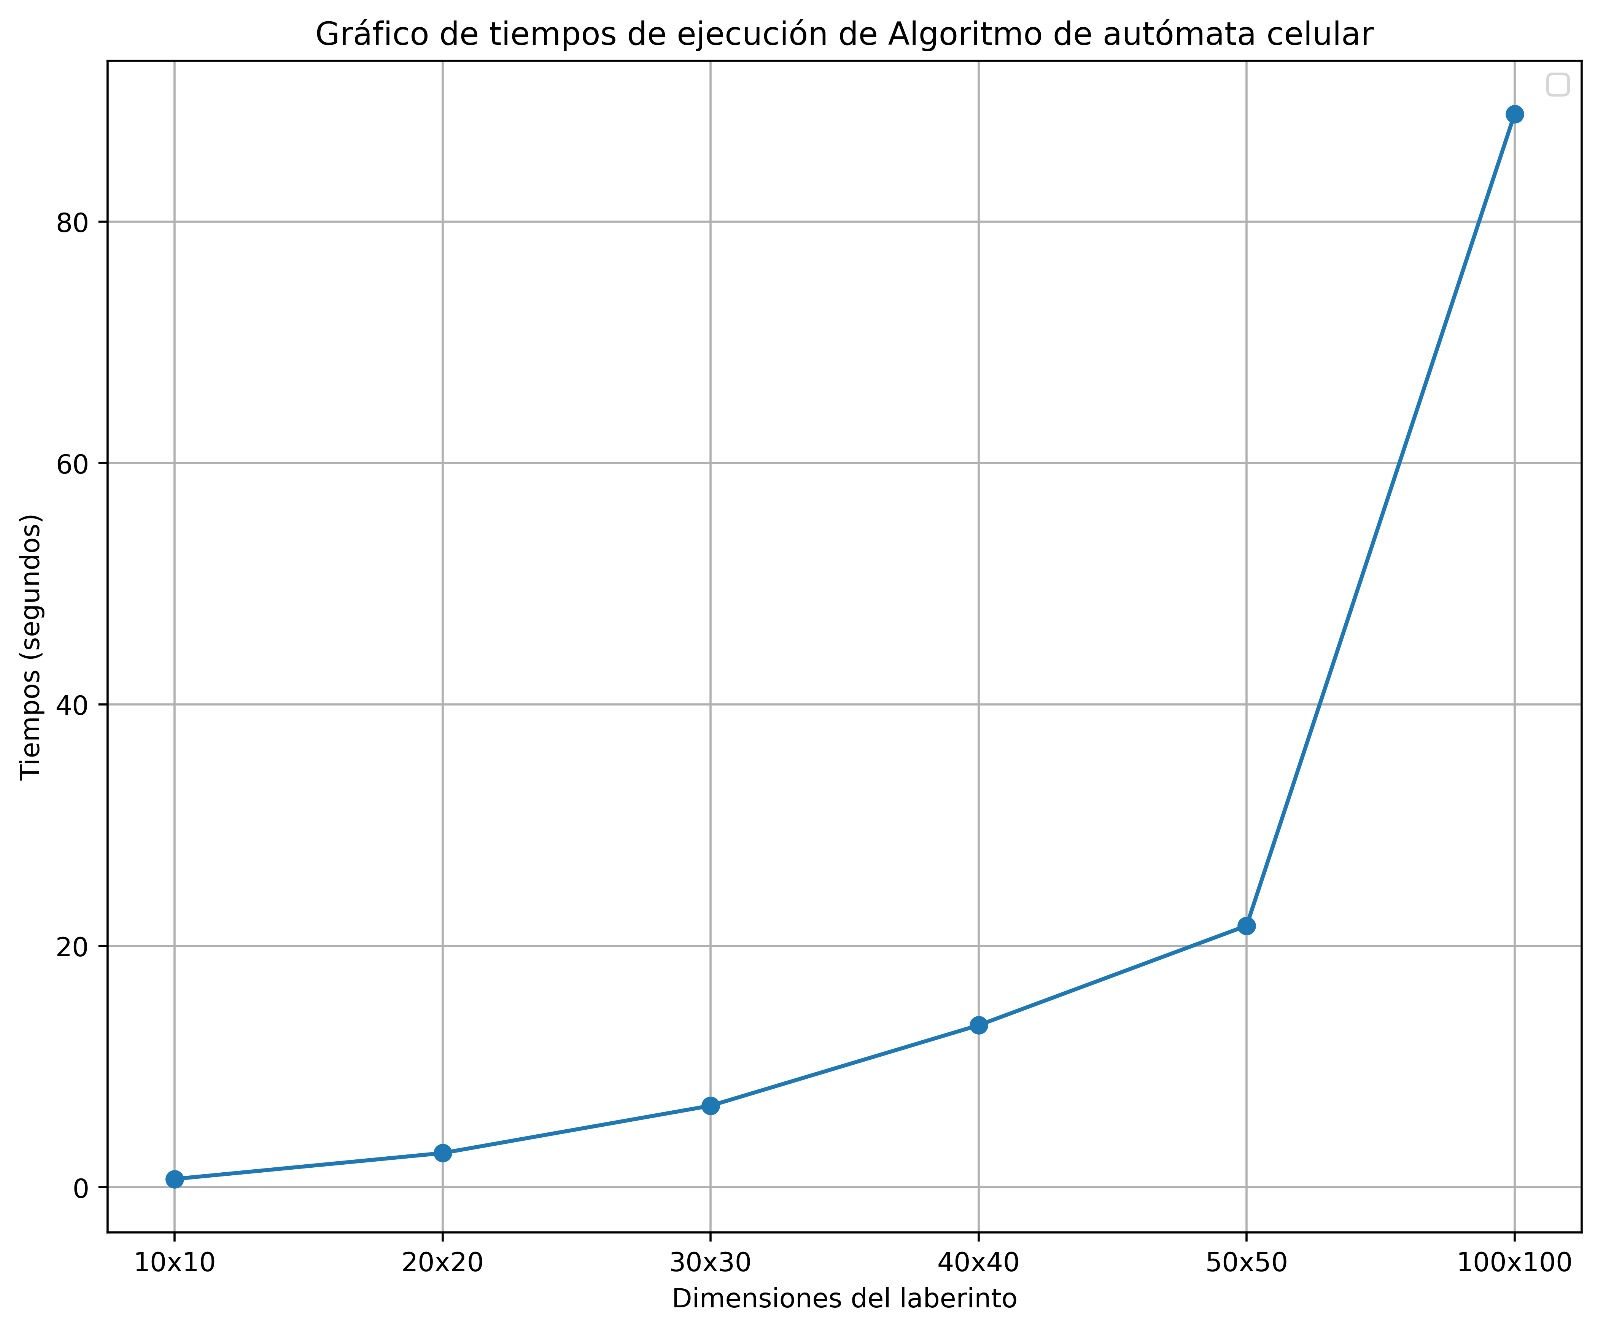
\includegraphics[width=\textwidth]{img/CelularTiempos.jpeg}  
    \caption{Gráfico de tiempos de ejecución de DungeonCelullar.}  
    \label{fig:CelularTiempos}
\end{figure}

\begin{figure}
    \centering  
    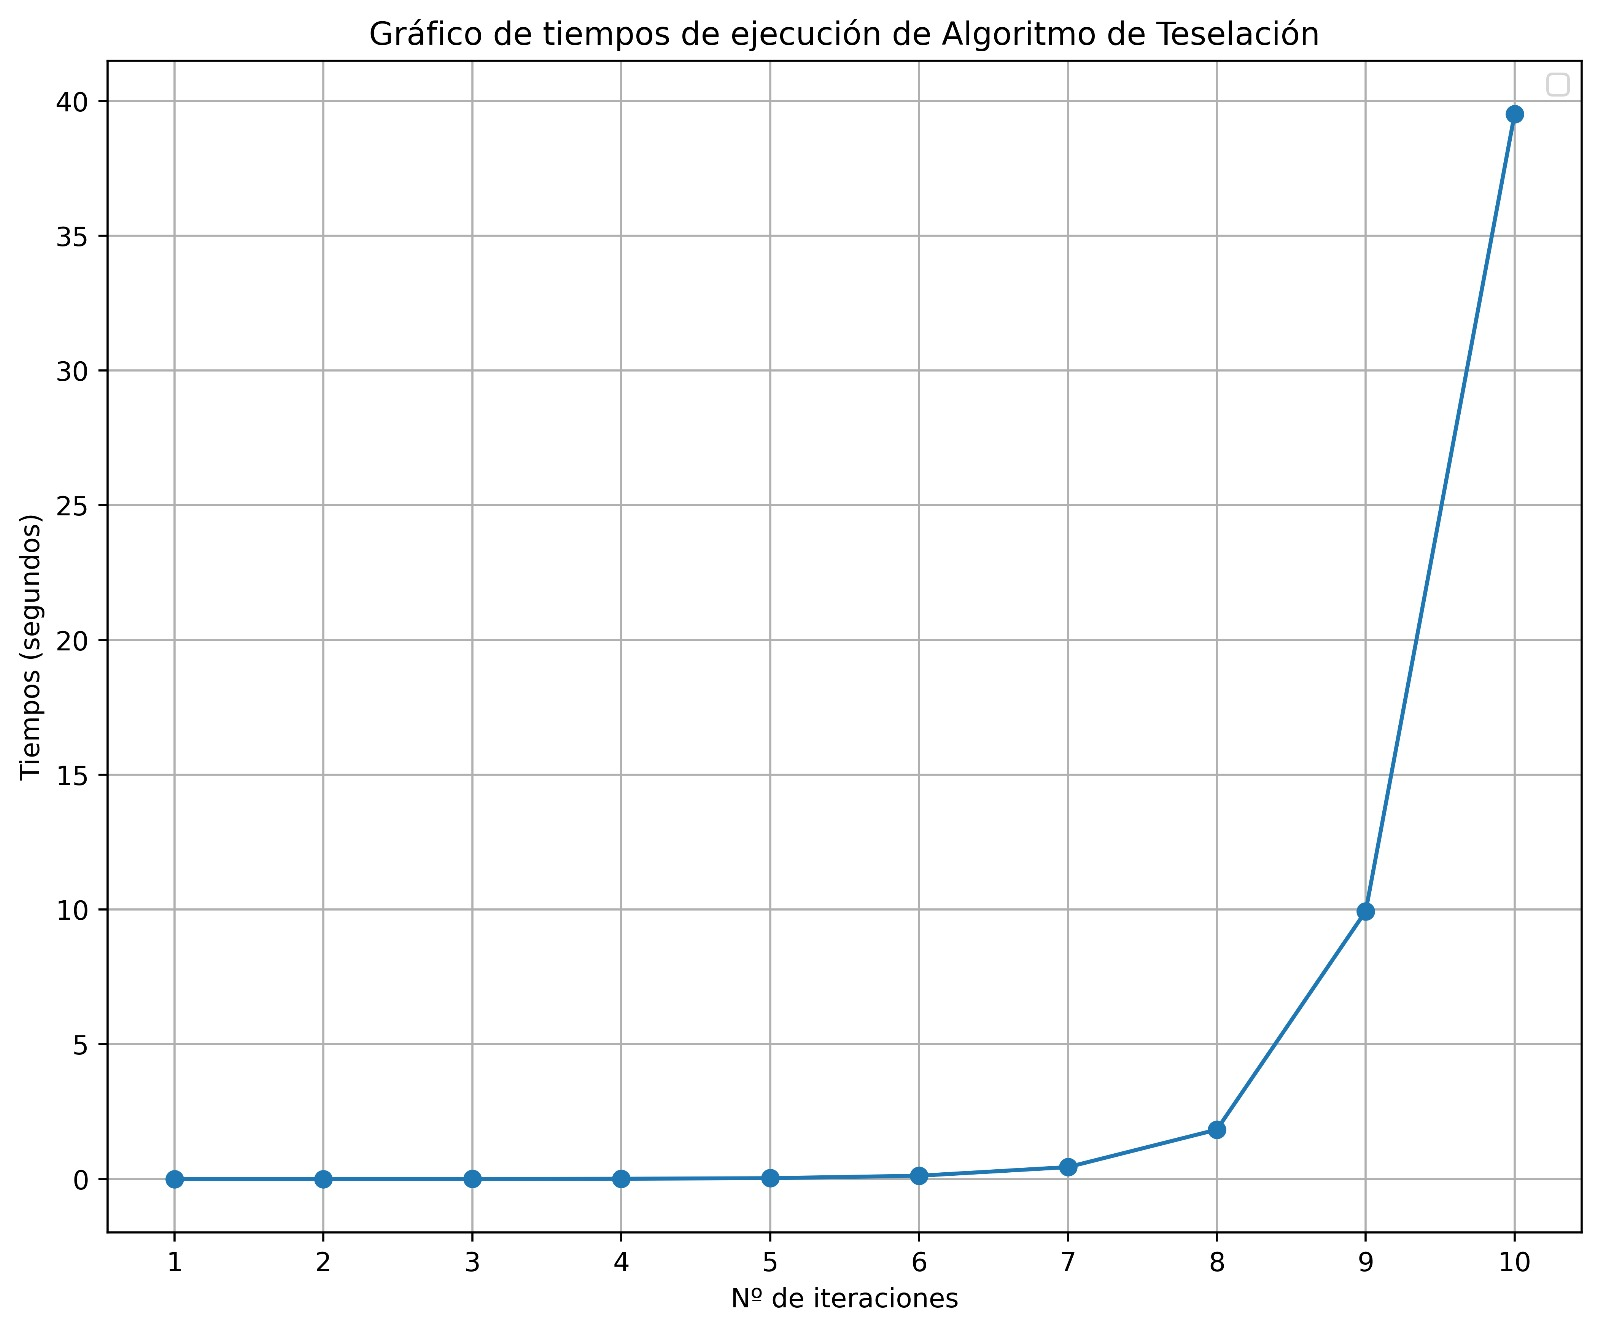
\includegraphics[width=\textwidth]{img/TeselacionTiempos.jpeg}  
    \caption{Gráfico de tiempos de ejecución de DungeonTesselation.}  
    \label{fig:TeselacionTiempos}
\end{figure}

\begin{table}
\centering
\caption{Resultados detallados de tiempos de ejecución de algoritmos (Parte 1)}
\label{tab:resultados_detallados_parte1}
\begin{tabular}{lrrr}
\toprule
          Algoritmo &    10x10 &    20x20 &    30x30 \\
\midrule
DungeonAldousBroder & 0.000524 & 0.005217 & 0.029298 \\
        DungeonPrim & 0.000443 & 0.001009 & 0.002407 \\
  DungeonBinaryTree & 0.000108 & 0.000330 & 0.000840 \\
         DungeonDFS & 0.000161 & 0.000592 & 0.001549 \\
     DungeonKruskal & 0.000200 & 0.001580 & 0.003289 \\
       DungeonEller & 0.000220 & 0.001374 & 0.005380 \\
\bottomrule
\end{tabular}
\end{table}

\begin{table}
\centering
\caption{Resultados detallados de tiempos de ejecución de algoritmos (Parte 2)}
\label{tab:resultados_detallados_parte2}
\begin{tabular}{lrrr}
\toprule
          Algoritmo &    40x40 &    50x50 &  100x100 \\
\midrule
DungeonAldousBroder & 0.027014 & 0.021885 & 0.136055 \\
        DungeonPrim & 0.004057 & 0.006651 & 0.026567 \\
  DungeonBinaryTree & 0.001427 & 0.002176 & 0.007692 \\
         DungeonDFS & 0.002483 & 0.004625 & 0.041779 \\
     DungeonKruskal & 0.006238 & 0.012281 & 0.138475 \\
       DungeonEller & 0.014307 & 0.032310 & 0.483169 \\
\bottomrule
\end{tabular}
\end{table}
